\documentclass[12pt]{article}

\usepackage{sbc-template}

\usepackage{graphicx,url}

%\usepackage[brazil]{babel}   
\usepackage[utf8]{inputenc}  

     
\sloppy

\title{Comparação entre os Algoritmos Branch and Bound, Christofides e Twice Around the Tree para o Problema do Caixeiro Viajante}

\author{Alex Eduardo\inst{1}, Murilo Ribeiro\inst{2}}


\address{Departamento de Ciência da Computação -- Universidade Federal de Minas Gerais
  (UFMG)\\
  Belo Horizonte -- MG -- Brazil
}

\begin{document} 

\maketitle

     
\begin{resumo} 
O Trabalho Prático II da disciplina de Algoritmos II teve como objetivo familiarizar os estudantes com o tratamento de problemas difíceis, mais especificamente na implementação dos algoritmos de \texttt{branch-and-bound} e dos algoritmos aproximativos \texttt{twice-around-the-tree} e de \texttt{Christofides}, utilizados na resolução do problema do caixeiro viajante.

A ideia geral do projeto é, além de fazer as implementações, compreender como os resultados variam conforme mudamos os algoritmos, o tamanho das instâncias e os tipos de distância entre os pontos gerados no plano bidimensional.
\end{resumo}


\section{Introdução}
O problema do caixeiro viajante (TSP, do inglês \textit{Travelling Salesman Problem}) é um dos problemas mais estudados na área da ciência da computação. A versão clássica do problema consiste em encontrar o menor caminho que percorra um conjunto de cidades, visitando cada uma exatamente uma vez e retornando à cidade inicial.

Neste trabalho, lidamos com instâncias geométricas do TSP, nas quais os vértices do grafo representam pontos em um plano euclidiano bidimensional, e as arestas correspondem às distâncias euclidianas entre esses pontos.

Foram utilizados conjuntos de dados do repositório TSPLIB95, disponível em \url{http://comopt.ifi.uni-heidelberg.de/software/TSPLIB95/}. Esses conjuntos consistem em diversas instâncias do TSP com diferentes configurações, permitindo a análise de desempenho dos algoritmos implementados.

\section{Implementação}

Os algoritmos foram implementados na linguagem Python, utilizando as bibliotecas \texttt{networkx} e \texttt{numpy}. A biblioteca \texttt{networkx} foi empregada para a criação e manipulação de grafos, enquanto \texttt{numpy} auxiliou no armazenamento eficiente de estruturas de dados e na realização de operações matemáticas.

As implementações incluem três principais abordagens para resolver o TSP:

\begin{itemize}
  \item \textbf{Branch-and-Bound}: Método exato que explora todas as possibilidades para encontrar a solução ótima, utilizando poda para reduzir o espaço de busca.
  \item \textbf{Twice Around the Tree}: Algoritmo aproximativo que constrói uma solução a partir de uma árvore geradora mínima.
  \item \textbf{Christofides}: Algoritmo aproximativo que utiliza uma combinação de árvore geradora mínima e emparelhamento perfeito.
\end{itemize}

Métricas como tempo de execução, consumo de memória e fator de aproximação foram coletadas durante os experimentos.

\section{Branch And Bound}

O método \texttt{branch-and-bound} busca a solução ótima do TSP por meio de uma abordagem sistemática de exploração do espaço de busca. A cada passo, o algoritmo divide o problema em subproblemas menores (branch) e utiliza limites inferiores para descartar subproblemas que não podem conter a solução ótima (bound).

A implementação exigiu a definição de funções de cálculo de limites inferiores eficientes, bem como estratégias de ordenação para explorar primeiro os subproblemas mais promissores. Embora produza soluções ótimas, o \texttt{branch-and-bound} é limitado em instâncias de grande porte devido ao crescimento exponencial do espaço de busca. Sendo assim somente foi possivel realizar o teste em uma instancia criada especificamente para ele que tivesse no máximo 16 pontos.

\section{Twice Around the Tree}

O algoritmo \texttt{Twice Around the Tree} é uma abordagem aproximativa para o TSP. Ele funciona da seguinte maneira:

\begin{enumerate}
  \item Constrói-se uma árvore geradora mínima (MST, do inglês \textit{Minimum Spanning Tree}) do grafo dado.
  \item Percorre-se todas as arestas da MST duas vezes para gerar um passeio fechado.
  \item Remove-se arestas repetidas no percurso, formando um ciclo hamiltoniano.
\end{enumerate}

A simplicidade do algoritmo o torna eficiente em termos de tempo de execução, mas a qualidade da solução pode variar dependendo da estrutura do grafo. Em geral, o fator de aproximação é 2 vezes a solução ótima.

\section{Christofides}

O algoritmo de \texttt{Christofides} é uma melhoria sobre o \texttt{Twice Around the Tree}, garantindo um fator de aproximação de 1,5 vezes a solução ótima em grafos completos com pesos que obedecem à desigualdade triangular. O algoritmo consiste nos seguintes passos:

\begin{enumerate}
  \item Construir uma árvore geradora mínima do grafo.
  \item Encontrar os vértices de grau ímpar na árvore e resolver o problema de emparelhamento mínimo perfeito para esses vértices.
  \item Combinar as arestas da árvore com o emparelhamento mínimo para formar um multigrafo euleriano.
  \item Encontrar um circuito euleriano e transformá-lo em um ciclo hamiltoniano eliminando vértices repetidos.
\end{enumerate}

Embora mais complexo que o \texttt{Twice Around the Tree}, o algoritmo de Christofides produz soluções de melhor qualidade, justificando seu uso em aplicações práticas.

\section{Análise de Resultados}

Os experimentos foram realizados utilizando instâncias do TSPLIB95, variando o número de vértices e os tipos de distâncias (euclidiana, Manhattan, etc.).

Os resultados mostraram que:
\begin{itemize}
  \item O \texttt{branch-and-bound} apresenta excelente precisão, mas é inviável para instâncias maiores devido ao tempo de execução elevado.
  \item O \texttt{Twice Around the Tree} é eficiente, mas produz soluções de menor qualidade em comparação ao Christofides.
  \item O algoritmo de \texttt{Christofides} oferece um bom equilíbrio entre qualidade da solução e tempo de execução, sendo mais adequado para aplicações práticas.
\end{itemize}



\begin{figure}[ht]
\centering
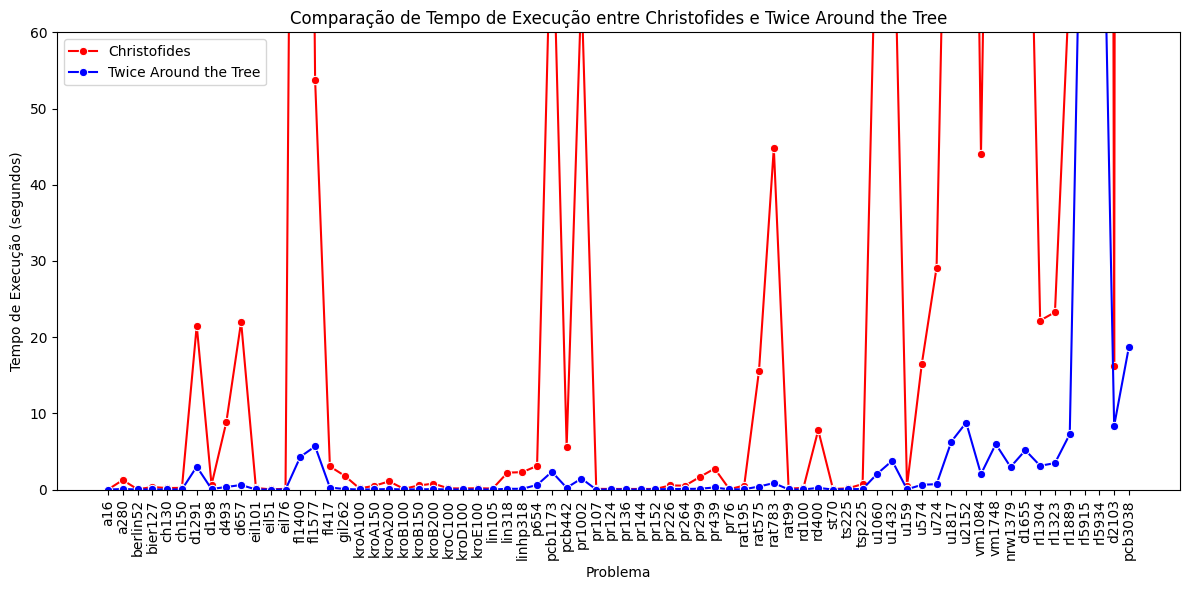
\includegraphics[width=.8\textwidth]{exec_time_comparison.png}
\caption{Comparação de Tempo de Execução entre Christofides e Twice Around the Tree. O algoritmo de Christofides apresenta tempos de execução muito maiores em diversos casos, mas em exemplos pequenos roda em poucos segundos como o Twice Around the Tree.}
\label{fig:execTimeComparison}
\end{figure}

\begin{figure}[ht]
\centering
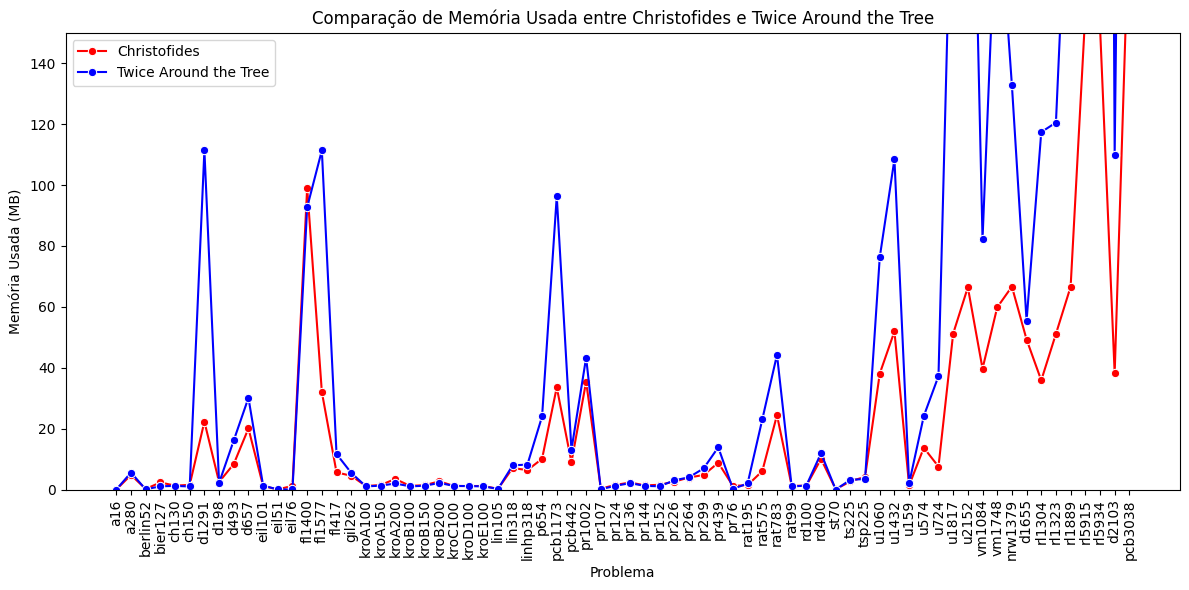
\includegraphics[width=.8\textwidth]{memory_usage_comparison.png}
\caption{Comparação de Memória Usada entre Christofides e Twice Around the Tree. O uso de memória entre os algoritmos é bem parecido na maioria dos testes, mas em alguns o Twice Around the Tree usa mais.}
\label{fig:memoryUsageComparison}
\end{figure}

\begin{figure}[ht]
\centering
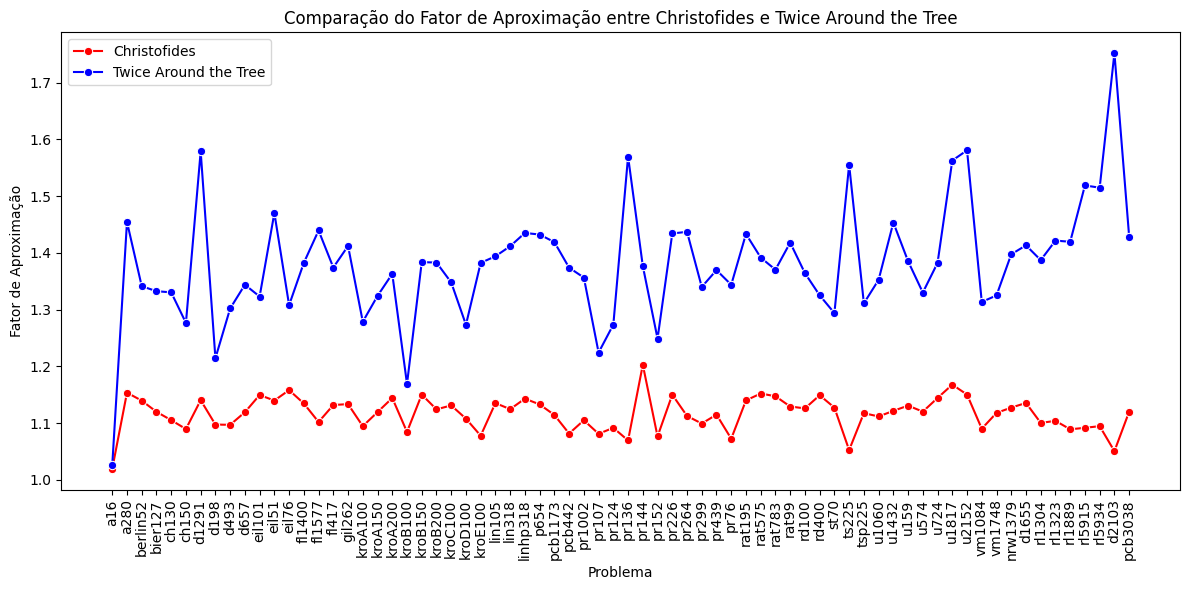
\includegraphics[width=.8\textwidth]{approximation_factor_comparison.png}
\caption{Comparação do Fator de Aproximação entre Christofides e Twice Around the Tree. O Christofides leva vantagem em todos os casos, tendo um fator de aproximação bem menor que o Twice Around the Tree.}
\label{fig:approximationFactorComparison}
\end{figure}

\begin{figure}[ht]
\centering
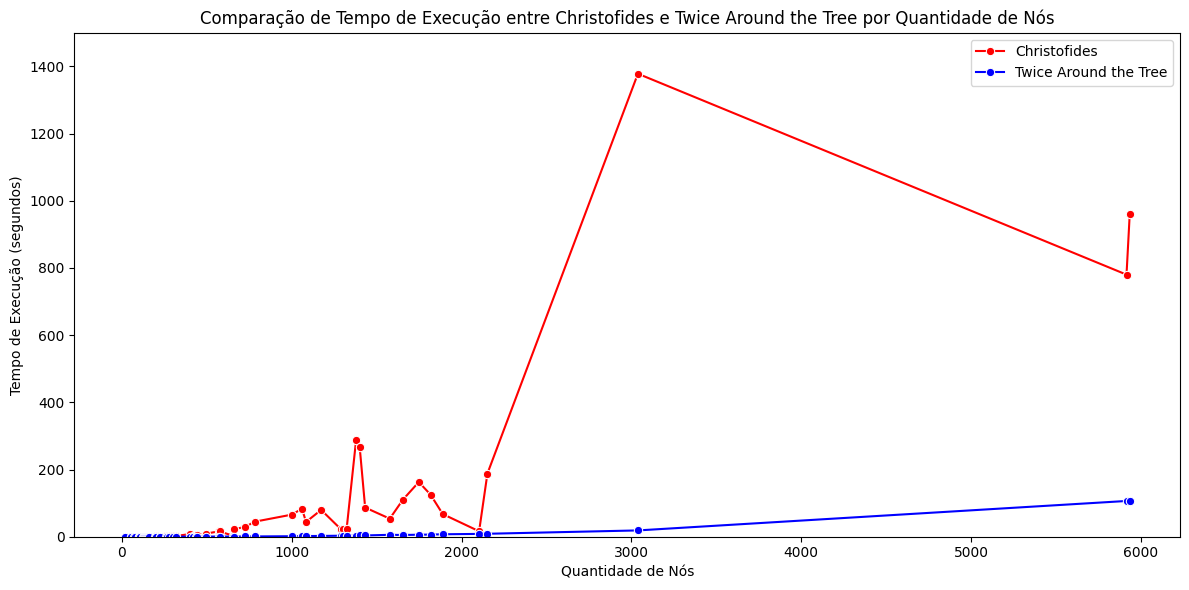
\includegraphics[width=.8\textwidth]{exec_time_nodes_comparison.png}
\caption{Comparação de Tempo de Execução entre Christofides e Twice Around the Tree por Quantidade de Nós. Quando a quantidade de nós cresce, o Christofides demora muito mais.}
\label{fig:execTimeNodesComparison}
\end{figure}

\begin{figure}[ht]
\centering
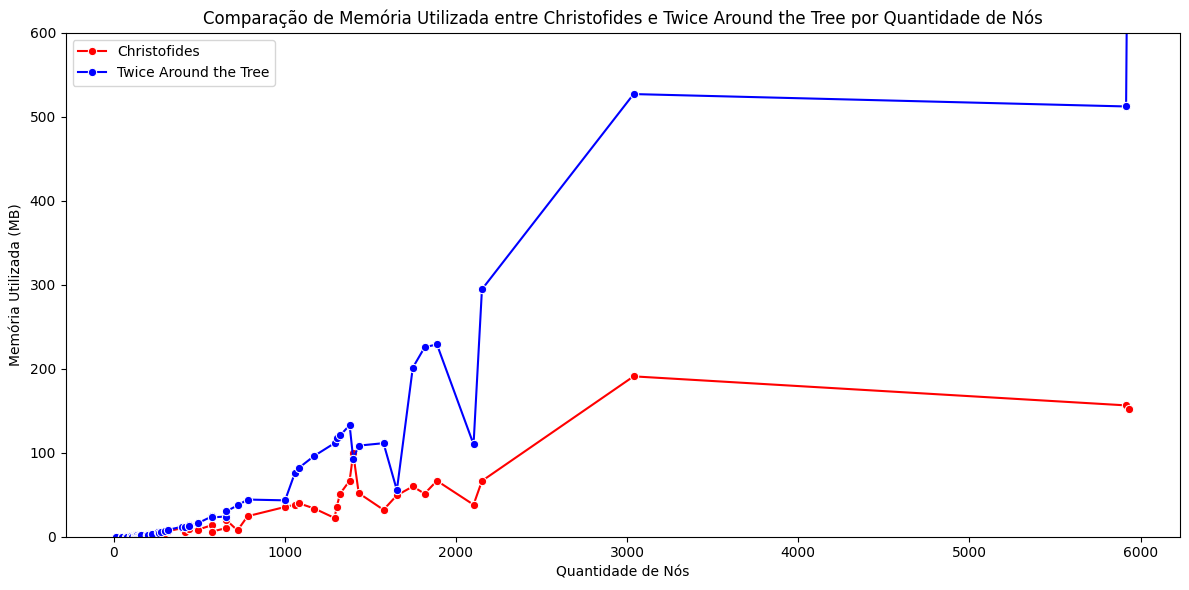
\includegraphics[width=.8\textwidth]{memory_usage_nodes_comparison.png}
\caption{Comparação de Memória Utilizada entre Christofides e Twice Around the Tree por Quantidade de Nós. O uso de memória entre os dois cresce quase na mesma velocidade, mas o Twice Around the Tree gasta mais, especialmente em casos com muitos nós.}
\label{fig:memoryUsageNodesComparison}
\end{figure}
\clearpage
\section{Conclusão}

O segundo trabalho prático teve como objetivo principal familiarizar os alunos com a resolução de problemas desafiadores. Inicialmente, é importante destacar como a execução de um algoritmo com complexidade exponencial contribuiu para entender as limitações desses algoritmos. O fato de o algoritmo de \texttt{branch-and-bound} ser impraticável para instâncias com 2$^{5}$ ou mais vértices evidenciou a vantagem dos algoritmos polinomiais, que são muito mais viáveis de serem aplicados.

Os outros dois algoritmos implementados, embora não ofereçam uma solução ótima, apresentam um tempo de execução significativamente menor, tornando-os mais adequados para instâncias reais que envolvem mais de 100.000 vértices.

Outro aspecto relevante do trabalho foi a maneira inteligente de abordar problemas difíceis, visando tornar suas soluções mais viáveis. A ideia de construir um algoritmo aproximativo era um tanto confusa antes do trabalho, mas ao observar os resultados obtidos, ficou claro como esses algoritmos funcionam de forma eficaz e por que são amplamente utilizados por pesquisadores.

Em síntese, o trabalho foi fundamental para uma compreensão mais aprofundada da matéria e ofereceu uma visão valiosa sobre algoritmos e resolução de problemas, com aplicação em diversas outras áreas.

\section{Referências}

\begin{thebibliography}{99}

\bibitem{knuth:84} Knuth, D. E. \textit{The Art of Computer Programming}. Addison-Wesley, 1984.

\bibitem{levitin:2011} Levitin, A. \textit{Introdução aos Algoritmos}. Pearson Prentice Hall, 2011.

\bibitem{wikipedia:travelling_salesman} Wikipedia contributors. \textit{Travelling salesman problem}. Disponível em: \url{https://en.wikipedia.org/wiki/Travelling_salesman_problem}. Acesso em: 2025.

\bibitem{video:travelling_salesman} UFC. \textit{Algoritmos Aproximativos - UFC - Caixeiro Viajante Métrico}. Disponível em: \url{https://www.youtube.com/watch?v=CmalaR7mNfk}. Acesso em: 2025.

\end{thebibliography}

\end{document}
